% ===================================================================
% Arquivo: capitulos/parte-III-pilares/cap-06-retropropagacao-e-gradiente.tex
% ===================================================================

\chapter{O Algoritmo da Repropropagação e Os Otimizadores Baseados em Gradiente}
\label{cap:retropropagacao-gradiente}

% ===================================================================
% Resumo do capítulo
% ===================================================================

% ===================================================================
% Método do Gradiente Descendente
% ===================================================================

\section{O Método do Gradiente Descendente}

O Método do Gradiente faz parte de uma série de métodos numéricos que possuem como função otimizar diferentes funções. Métodos dessa forma veem sendo estudados a séculos, um exemplo disso é o trabalho \textit{\citetitle{CauchyMetodoDoGradiente}} (Método geral para resolução de sistemas de equações simultâneos em portguês) do matemático francês do século XVIII \textcite{CauchyMetodoDoGradiente}, em que o autor apresenta um método que pode ser considerado um precursor para o método do gradiente atual.

Nesse texto, o autor apresenta uma forma de minimizar uma função de múltiplas variáveis ($u=f(x,y,z)$) que não assume valores negativos, para fazer isso, ele faz uso do cálculo de derivadas parciais dessa função de cada um dos seus componentes ($D_x u, D_y u, D_z u$), em seguida, ele realiza um passo de atualização, de forma que os os valores de cada uma das variáveis sejam ligeiramente incrementados por valores ($\alpha, \beta, \gamma$) \parencite{CauchyMetodoDoGradiente}. Um ponto importante destacado por \textcite{CauchyMetodoDoGradiente} é de que esses incrementos devem ser proporcionais ao negativo das suas respectivas derivadas parciais, ele descreve que esse processo de calcular as derivadas e fazer pequenos incrementos deve ser feito de forma iterativa, assim, calculá-se as derivadas, faz-se os incrementos, e o passo é repetido até convergir para o valor mínimo de $u$.

Esse trabalho explica bem como aplicar o método do gradiente para se calcular mínimos de funções, mas para facilitar o entendimento do leitor, em seguida está um exemplo ilutrativo explicando o funcionamento dessa ferramenta.

\subsection{Exemplo Ilustrativo: Cadeia de Montanhas}

Imagine que você adora aventuras, e por isso, decidiu fazer uma trilha em uma floresta que fica em uma cadeia de montanhas que podem ser escaladas. Então, você teve a incrivel ideia de ir para o menor ponto dessa cadeia de montanhas, pois, no guia que você estava seguindo, falava que lá havia um lago com uma água cristalina, perfeito para tirar fotos.

Para chegar até esse lago, você conta com uma bússula um tanto quanto diferente, ao invés dela apontar para o norte como uma bússola comum, ela aponta para a direção do lugar com menor altitude de uma região. Isso é perfeito para o que você precisa, pois ela irá apontar justamente para o lago de você quer ir.

Com isso em mente, você criou um plano de como irá chegar a esse lago, ele é método que segue dois passos diferentes, sendo eles:

\begin{enumerate}
    \item Olha na bússola qual a direção ela está apontando;
    \item Anda um metro na direção apontada pela bússola.
\end{enumerate}

Você chegou na conclusão que se seguir essa estratégia repetidas vezes, em algum momento, você inevitavelmente irá chegar no lago que está querendo tirar as suas fotos.

Na matemática, existe um método semelhante a este, que busca com base em uma bússola (chamada de vetor gradiente), encontrar um ponto de mínimo de um determinado lugar (neste caso, uma função composta por múltiplas variáveis). Esse é o método do gradiente, ele é ponto central desse capítulo, pois, ele (e suas variações) junto com o algortimo da retroprogação são algumas das principais ferramentas que colaboram para que os modelos de aprendizado de máquina possam aprender com os seus erros e com isso se tornarem melhores a cada iteração.

\subsection{O Método em Si}

A vantagem do método do gradiente é que ele é uma ferramenta matemática, e por isso pode ser representado utilizando notações mais formais e de forma enxuta. As notações utilizadas por Cauchy são diferentes das que são utilizadas hoje em dia, mas o seu significado não muda. Em \citetitle{DeepLearningBook}, \textcite{DeepLearningBook} explicam essa ferramenta através da equação \ref{eq:metodo-do-gradiente} que deve ser repetida por múltiplos passos até o modelo convergir, ou seja, encontrar o ponto de mínimo da função estudada.

\begin{equacaodestaque}{Método do Gradiente Descendente}
    x' = x - \epsilon \nabla f(x)
    \label{eq:metodo-do-gradiente}
\end{equacaodestaque}

Em que:

\begin{itemize}
    \item $x'$: representa as coordenadas do próximo ponto;
    \item $x$: representa as coordernadas do ponto atual;
    \item $\epsilon$: representa o tamanho do passo, também chamado de taxa de aprendizado;
    \item $\nabla f(x)$: representa o vetor gradiente calculado na posição do ponto atual ($x$) para função que se deseja otimizar.
\end{itemize}

Note que assim como no método proposto por Cauchy, é pego como base o inverso do vetor gradiente. Isso ocorre pois o vetor gradiente é um vetor especial que tem como principal propriedade apontar para a direção de maior crescimento de uma função no ponto que está sendo calculada. Mas no método, o objetivo não é encontrar o ponto que irá gerar os maiores valores da função, e sim o contrário. Por isso, é tomado inverso do vetor gradiente, que, dessa forma, estará então apontando para a direção de menor crescimento de uma função.

Um ponto a ser destacado nesse metodo é na hora de escolher uma taxa de aprendizado para ser utilizada no método. Uma taxa de aprendizado muito pequena signifca que o passo que o modelo irá dar de um ponto para outro será menor, e com isso implica que ele levará mais passos para encontrar um ponto de mínimo. É como se você fosse comparar a quantidade de passos que você gasta para andar do seu quarto até a sua cozinha com a quantidade de passos dados por uma formiga até lá, ambos vão chegar no local, mas a formiga certamente irá demorar bem mais. Considerando isso, surge então a hipótese de que quanto maior for o passo, mais rápido será a convergência, mas isso também não funciona muito bem, pois um passo muito largo pode ultrapassar o ponto de mínimo indo parar em outro canto da função, e ficará tentando chegar até o mínimo mas não irá conseguir pois caminha uma distância muito grande de uma só vez. Essas duas situações, em que o passo é pequeno demais e que o passo e grande demais, são ilustradas na figura \ref{fig:comparativo-tamanho-do-passo}.

\begin{figure}[h!]
    \centering
    \includegraphics[width=1\linewidth]{../imagens/retropropagacao-gradiente/comparativo-de-passos.png}
    \caption{Comparativo do tamanho de passos em uma função polinomial.}
    \label{fig:comparativo-tamanho-do-passo}
\end{figure}

Na prática, escolher o valor da taxa de aprendizado é uma tarefa que irá depender de modelo em modelo, também irá variar com os diferentes métodos de otimização além da topologia da rede neural que está sendo construída. É sempre recomendado então experimentar diferentes tamanhos de passo, de forma que seja encontrado um que melhor se ajusta ao cenário que está sendo trabalhado.

Outro ponto que deve-se atentar é com relação as funções que estão sendo analisas ao utilizar o método do gradiente mas também qualquer otimizador que seja baseado nele. Se tivermos uma função convexa, em que seu formato lembra um funil, será bem mais fácil para o modelo encontrar o ponto de mínimo global daquela função. Mas se tivermos uma função não convexa, cheia de ondas e com muitos pontos de mínimos locais e pontos de sela, a convergência do modelo será pior, pois existe a chance de que ele fique preso em um ponto de mínimo local ou em um ponto de sela. Isso afeta diretamente o desempenho da rede neural que estará sendo criada, fazendo com que ela tenha métricas piores. O problema é que muitas das vezes a função $f(x)$ que estaremos interessados para calcular o desemepenho do modelo será não convexa, dificultando o seu aprendizado.

Na figura \ref{fig:funcao-convexa-nao-convexa} é possível ver o gráfico de duas funções diferentes, a primeira sendo uma função convexa e a segunda uma função não convexa.

\begin{figure}[h!]
\centering

% --- Gráfico 1: Função 3D Convexa ---
\begin{minipage}{0.48\textwidth}
    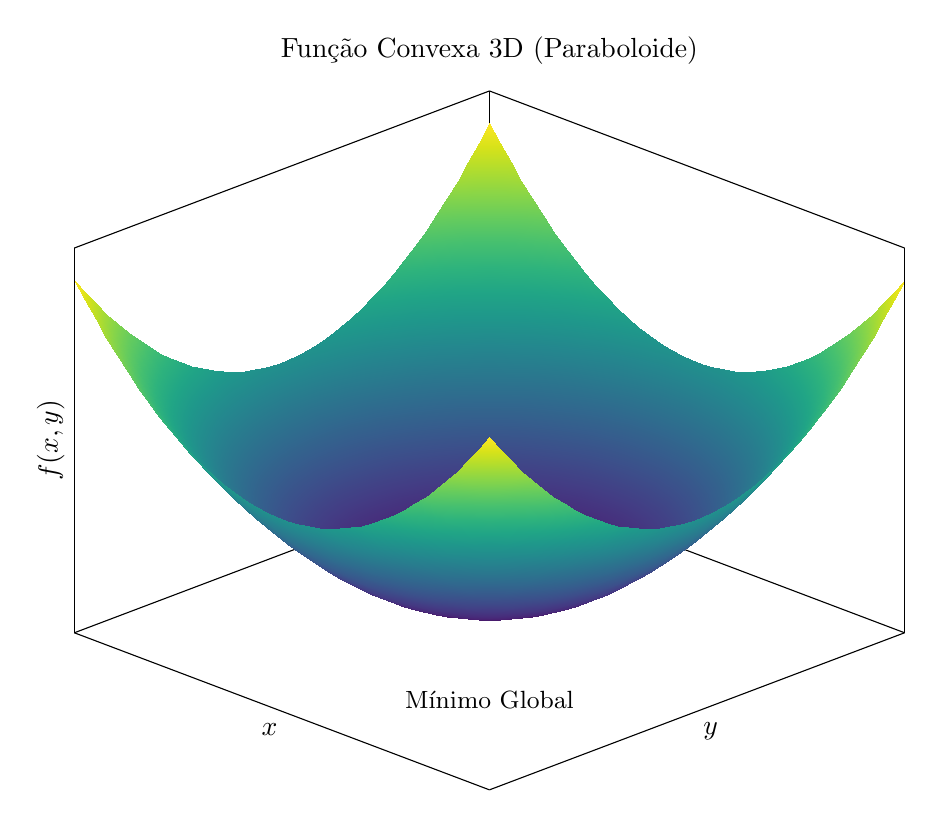
\begin{tikzpicture}
        \begin{axis}[
            title={Função Convexa 3D (Paraboloide)},
            xlabel=$x$,
            ylabel=$y$,
            zlabel={$f(x,y)$},
            xtick=\empty, ytick=\empty, ztick=\empty, % Remove marcações
            view={45}{30}, % Define o ângulo de visão 3D
            width=\textwidth,
            colormap/viridis, % Define o esquema de cores
        ]
        
        % Plot da superfície 3D z = x^2 + y^2
        \addplot3[
            surf, % Tipo de gráfico: superfície
            shader=interp, % Cores interpoladas para um visual suave
            domain=-2:2,
            domain y=-2:2,
            samples=40, % "Resolução" da malha
        ] {x^2 + y^2};
        
        % Marcador para o mínimo global
        \node at (axis cs:0,0,-2) [below, font=\small] {Mínimo Global};
        
        \end{axis}
        \label{fig:funcao-convexa}
    \end{tikzpicture}
\end{minipage}
\hfill % Espaço entre as figuras
% --- Gráfico 2: Função 3D Não-Convexa ---
\begin{minipage}{0.48\textwidth}
    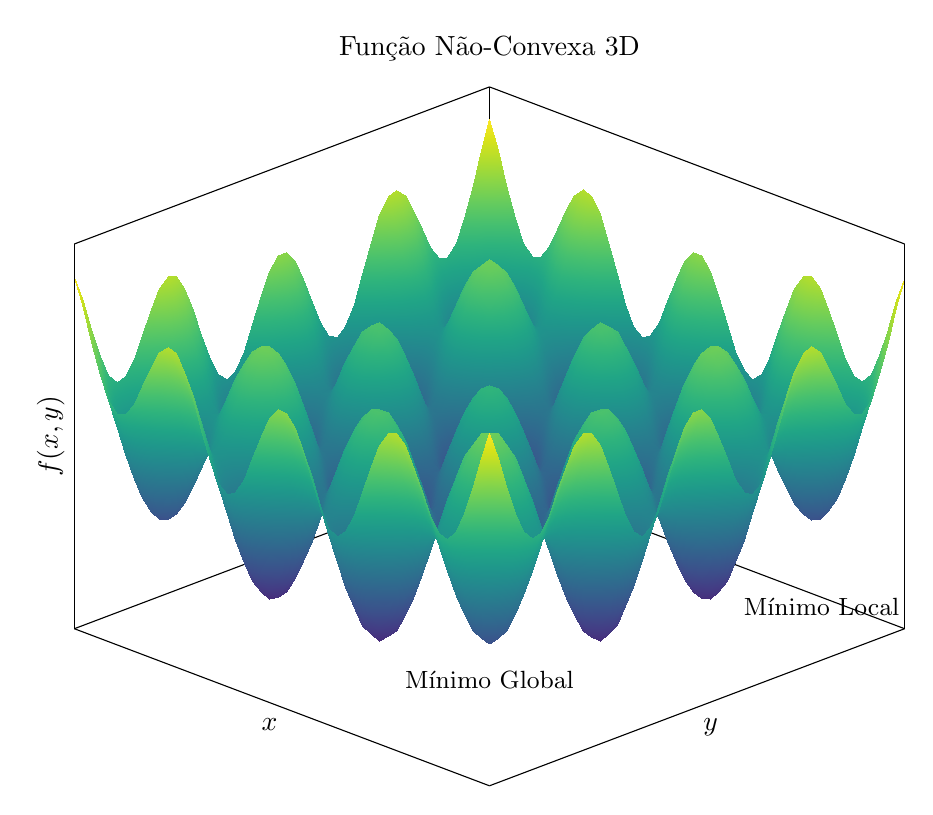
\begin{tikzpicture}
        \begin{axis}[
            title={Função Não-Convexa 3D},
            xlabel=$x$,
            ylabel=$y$,
            zlabel={$f(x,y)$},
            xtick=\empty, ytick=\empty, ztick=\empty,
            view={45}{30},
            width=\textwidth,
            colormap/viridis,
        ]
        
        % Plot da superfície com "ondinhas"
        % A função é um paraboloide + cossenos para criar as ondas
        \addplot3[
            surf,
            shader=interp,
            domain=-2.5:2.5,
            domain y=-2.5:2.5,
            samples=50,
        ] {(x^2+y^2)/5 + 2 - cos(deg(180*x)) - cos(deg(180*y))};
        
        % Marcadores para os mínimos
        \node at (axis cs:0,0,-1) [below, font=\small] {Mínimo Global};
        \node at (axis cs:2,2,0) [font=\small] {Mínimo Local};
        
        \end{axis}
        \label{fig-funcao-nao-convexa}
    \end{tikzpicture}
\end{minipage}
\caption{Comparação entre funções 3D convexas e não-convexas.}
\label{fig:funcao-convexa-nao-convexa}
\end{figure}

\subsection{Implementação em Python}

Para implementar o método do gradiente utilizando Python e a biblioteca de cálculos Numpy, deve-se seguir como base a equação \ref{eq:metodo-do-gradiente}, criando uma classe implenta essa ferramenta, recebendo como parâmetros de entrada a taxa de aprendizado, a função que se quer encontrar o ponto de mínimo, e um ponto inicial, que pode ser um conjunto de coordenadas aleatórias ou escolhidas pelo programador.

\begin{codelisting}{Classe completa do otimizador GradientDescent}{gd_class}
class GradientDescent:

    def __init__(self, function, function_prime, initial_point, learning_rate=0.001, max_iterations=100, tolerance=1e-6):
        self.f = function
        self.fp = function_prime
        self.ip = initial_point
        self.lr = learning_rate
        self.iterations = max_iterations
        self.tol = tolerance
        self.path = []

    def update_step(self):
        for i in range(self.iterations):
            self.path.append(self.ip)
            grad = self.fp(self.ip)
            if abs(grad) < self.tol: break
            self.ip = self.ip + self.lr * (-grad)
        return self.ip, self.path

\end{codelisting}

% ===================================================================
% A Retropropagação
% ===================================================================

\section{A Retropropagação: Aprendendo com os Erros}

Ainda no contexto de utilizar com o vetor gradiente para otimizar um modelo de rede neural, existe uma ferramenta que trabalha justamente com essse processo, ela é a retropropagação ou \textit{backpropagation} em inglês.

\begin{definicaomoderna}{\textbf{Definição:}}
A \textbf{retropropagação} é uma ferramenta que veio para permitir que redes que fazem o uso de unidades de neurônios possam aprender, para isso, o procedimento ajusta repetidamente os pesos das conexões da rede para minimizar a diferença entre o valor atual da saída do vetor da rede neural com o valor real desejado \parencite{BackpropagationArticle}.
\end{definicaomoderna}

Essa ferramenta foi introduzida para a comunidade científica pelos pesquisadores \textcite{BackpropagationArticle} no texto \textit{\citetitle{BackpropagationArticle}}, 

% ===================================================================
% Otimizadores Baseados em Gradiente
% ===================================================================

\section{Otimizadores Baseados em Gradiente}

\subsection{Método do Gradiente Estocástico}

\subsubsection{Implementação em Python}

\subsection{Método do Gradiente com Momentum}

\subsubsection{Implementação em Python}

\subsection{Nesterov}

\subsubsection{Implementação em Python}

\subsection{AdaGrad}

\subsubsection{Implementação em Python}

\subsection{RMSProp}

\subsubsection{Implementação em Python}

\subsection{Adam}

\subsubsection{Implementação em Python}

\subsection{Nadam}

\subsubsection{Implementação em Python}

% ===================================================================
% Método de Newton
% ===================================================================

\section{O Método de Newton: Indo Além do Gradiente}

\subsection{Implementação em Python}

